% !TEX root = ../agglo_clust_review.tex

\begin{figure}
        \centering
\begin{minipage}{0.45\textwidth}
\centering
        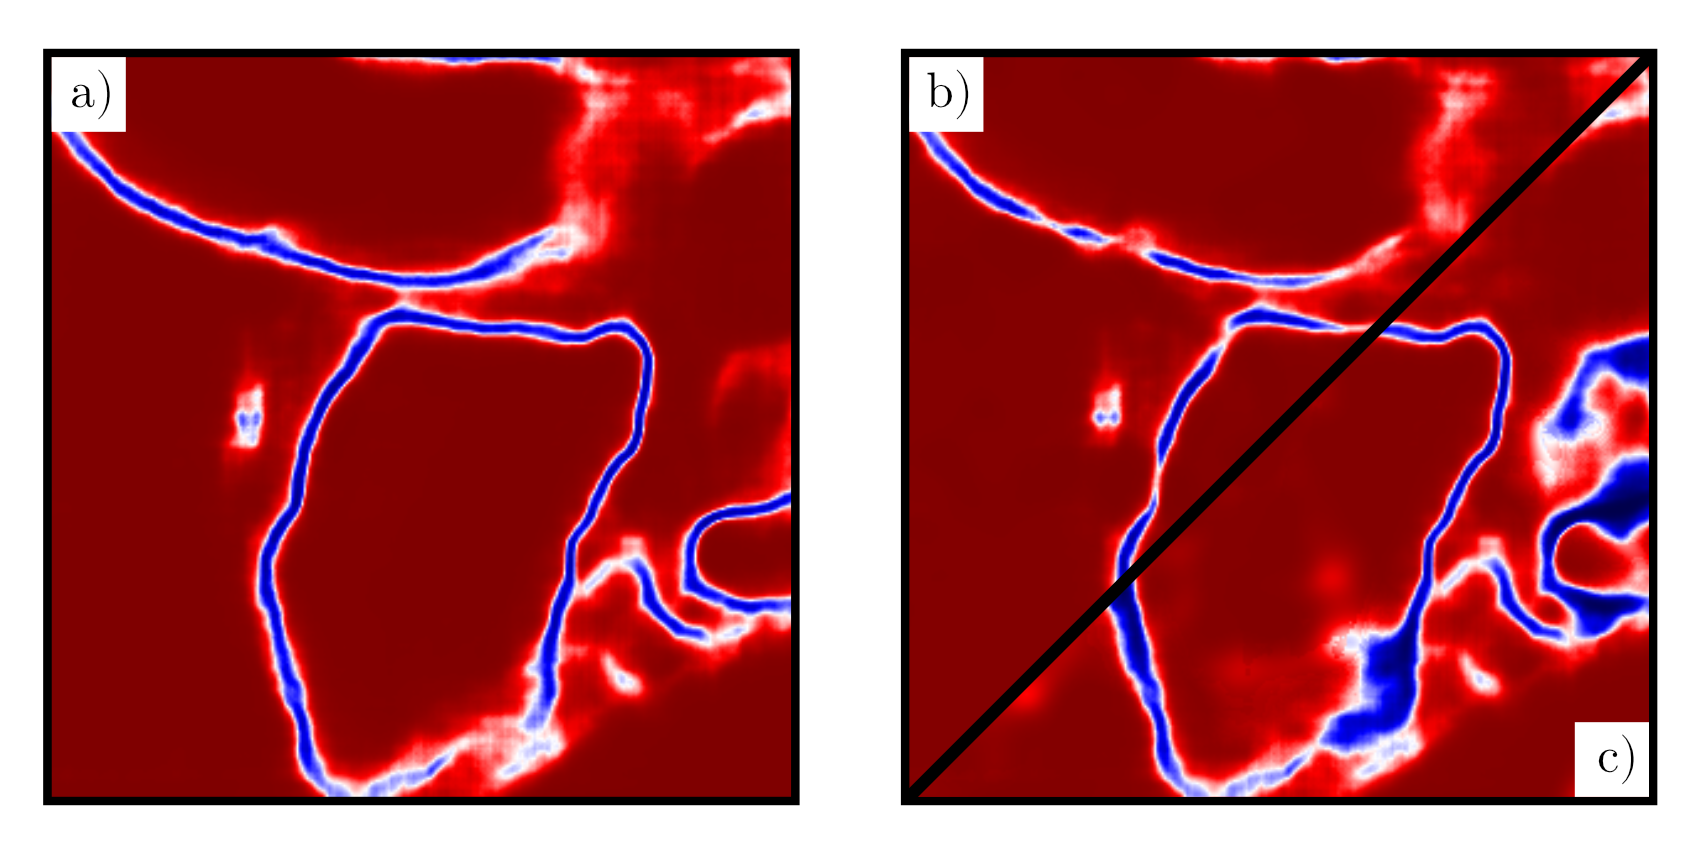
\includegraphics[width=0.85\textwidth,trim=0.1in 0.0in 0.05in 0.0in,clip]{figs/noisy_affs_comparison.png}
   
    \captionof{figure}{The two figures represent the CNN predictions on a slice of the neuron segmentation CREMI challenge \cite{cremiChallenge} with and without additional noise. Blue pixels represent boundary evidence. Image a) shows the original CNN predictions, b) the merge-biased version $\tilde{F}_{+}$ and c) the split-biased version $\tilde{F}_{-}$ (see definition \ref{eq:noise_biased_predictions}). 
    %The color of each pixel represents how probable it is for it to be in the same cluster with its neighboring pixel on the right (red: same cluster; blue: different ones). 
    %Adding merge-biased noise tends to create holes in the boundaries; split-biased noise add non-existing boundaries 
    }
    \label{fig:noisy_affs}
    \end{minipage}\hfill
\begin{minipage}{0.49\textwidth}
\centering
        % 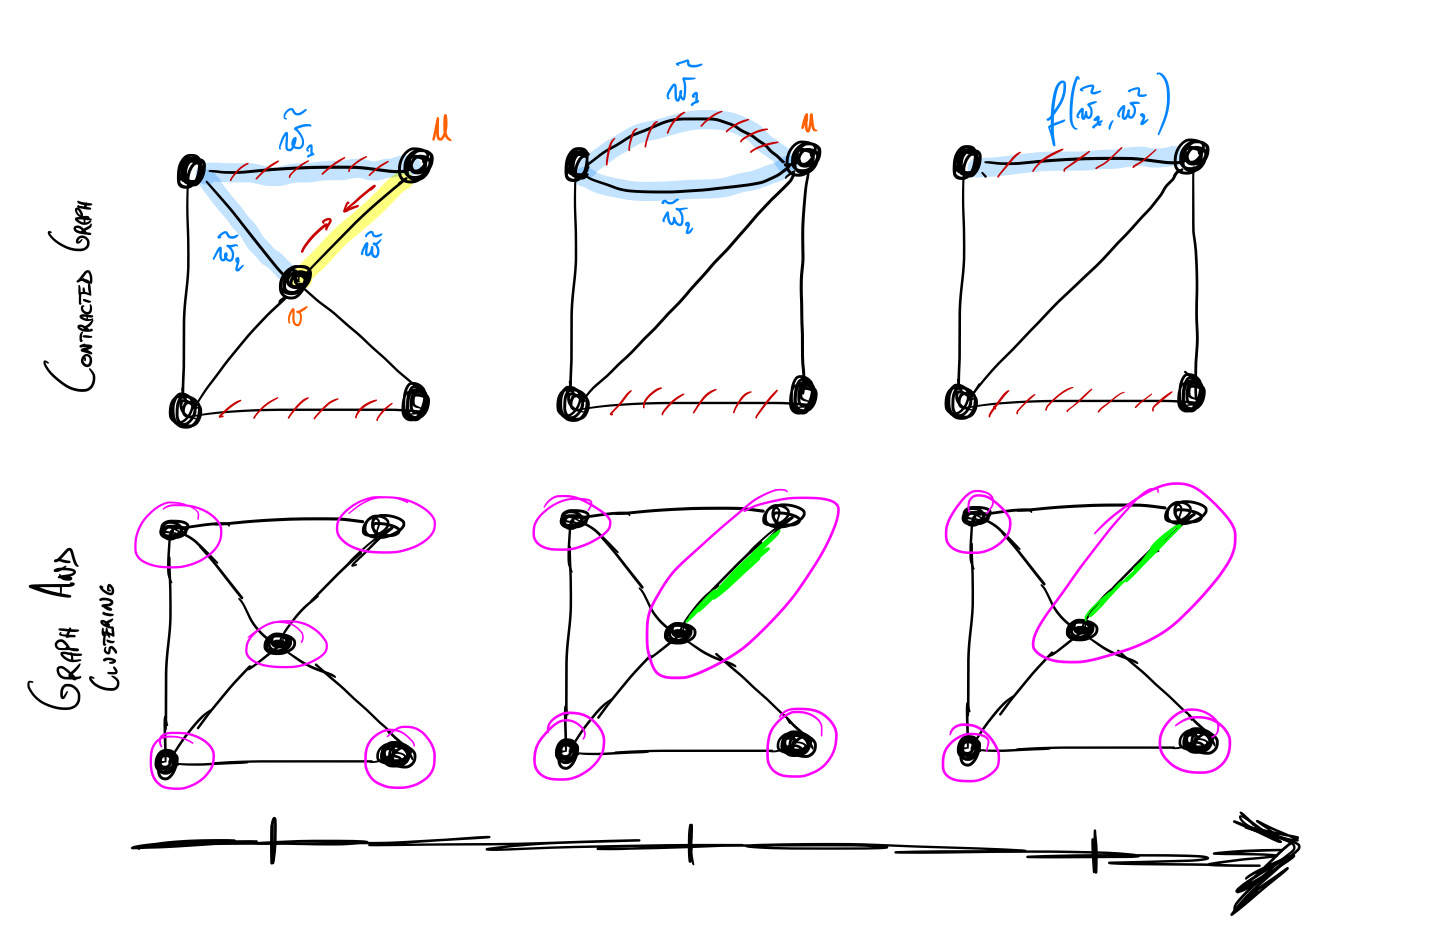
\includegraphics[width=\textwidth,trim=0.1in 0.4in 0.2in 0.2in,clip]{./figs/edge_contraction.png} % left bottom right top
        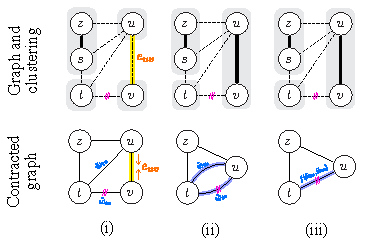
\includegraphics[width=\textwidth]{./figs/edge_contraction.pdf} % left bottom right top
\captionof{figure}{ 
{\small Example of edge contraction. First row: original graph $\mathcal{G}$; clustering $\Pi$ (gray shaded areas) with dashed edges on cut; cannot-link constraints (violet bars). Second row: contracted graph $\tilde{\mathcal{G}}_\Pi$. In step ii), edge $e_{uv}$ is contracted and node $v$ deleted from $\tilde{\mathcal{G}}_\Pi$. In step iii), double edges $e_{tu}$ and $e_{tv}$ resulting from edge contraction are replaced by single edge with updated interaction $f(\tilde{\cost}(e_{tu}), \tilde{\cost}(e_{tv}))$, see definitions in Tab.~\ref{tab:linkage-criteria}. }
\label{fig:edge_contraction_and_contr_graph}  }
    \end{minipage}
\end{figure}


\section{Supplementary Material}
\paragraph{Update rules} During the agglomerative process, the interaction between adjacent clusters has to be properly updated and recomputed.  % given by the linkage criterion defined in Sec. \ref{sec:notation} and
An efficient way of implementing these updates can be achieved by representing the agglomeration as a sequence of \emph{edge contractions} in the graph. Given a graph $\mathcal{G}(V,E,\cost)$ and a clustering $\Pi$, we define the associated \emph{contracted graph} $\tilde{\mathcal{G}}_\Pi(\tilde{V}, \tilde{E}, \tilde{\cost})$, such that $\tilde{V} \subseteq V$ and each node $u\in \tilde{V}$ represents the cluster $S_u \in \Pi$ including $u\in V$. Edges in $\tilde{E}$ represent adjacency-relationships between clusters and the signed edge weights $\tilde{\cost}_e$ are given by inter-cluster interactions $\tilde{\cost}(e_{uv})=\interact_{S_u,S_v}$. 
For the linkage criteria tested in this work, when two clusters $S_u$ and $S_v$ are merged, the interactions between the new cluster $S_u \cup S_v$ and each of its neighbors depend only on the previous interactions involving $S_u$ and $S_v$. Thus, we can easily recompute these interactions by using a simple \emph{update rule} $f$ that does not involve any loop over the edges of the original graph $\mathcal{G}$. As an example, given the single-linkage criterion defined in Eq. \ref{eq:max_linkage}, the interaction between $S_u \cup S_v$ and one of its neighbors $S_t$ is simply given by:
\begin{equation}
  \interact_{S_u \cup S_v,S_t} = f( \interact_{S_u,S_t}, \interact_{S_v,S_t}) = f(\tilde{\cost}(e_{ut}), \tilde{\cost}(e_{vt})) = \max \{ \tilde{\cost}(e_{ut}), \tilde{\cost}(e_{vt}) \}
\end{equation}
All the update rules tested in this article are listed in Table \ref{tab:linkage-criteria}.



\begin{itemize}
\item Equivalence Mutex Watershed and Greedy Edge Contraction
\item Complexity: plain agglo., addition of the cannot-link constraints and then comment about efficient implementation of MWS and of single-linkage (what about single linkage+CLC...?)
\item Noise: also mention details about plots (fix some long-range edges, fix noise seed and vary K)
\item exp. setup details: enforcing local merges, MWS distinguish between repulsive-long, post-processing of small segments, loss, architecture, training parameters, offset patterns
\item 

\end{itemize}

\begin{table*}
    \centering
    \begin{subtable}[t!]{0.98\textwidth}\centering
        \begin{tabular}{c| c | c| c | c | c | c | c}
Update rule & \makecell{Use Cannot-Link\\Constraints} & Log-costs & \makecell{Multicut objective} & Runtime (s) & ARAND & VI-merge & VI-split\\ \midrule\midrule
% \textbf{mean} & False & \textbf{-102739991} & {\color{Orange} 3797 } & {\color{ForestGreen} \textbf{0.0708} } & {\color{ForestGreen} 0.286 } & {\color{ForestGreen} 0.428 } \\
% % mean & False & -102730208 & {\color{Orange} 2562 } & {\color{ForestGreen} 0.0715 } & {\color{ForestGreen} 0.292 } & {\color{ForestGreen} 0.423 } \\
% MutexWatershed & False & -102313957 & {\color{ForestGreen} 830 } & {\color{ForestGreen} 0.0754 } & {\color{ForestGreen} 0.291 } & {\color{Orange} 0.471 } \\
% sum & False & -101846418 & {\color{Red} 12681 } & {\color{Orange} 0.1623 } & {\color{Orange} 0.427 } & {\color{ForestGreen} 0.427 } \\
% % sum & False & -101732952 & {\color{Red} 12287 } & {\color{Orange} 0.1624 } & {\color{Orange} 0.436 } & {\color{ForestGreen} 0.390 } \\
% sum & True & -101487448 & {\color{Red} 8497 } & {\color{Orange} 0.1626 } & {\color{Orange} 0.428 } & {\color{ForestGreen} 0.414 } \\
% % sum & True & -100745943 & {\color{Red} 13361 } & {\color{Orange} 0.1574 } & {\color{Orange} 0.410 } & {\color{Orange} 0.451 } \\
% mean & True & -100279671 & {\color{Orange} 4713 } & {\color{Orange} 0.1353 } & {\color{ForestGreen} 0.265 } & {\color{Red} 0.717 } \\
% % mean & True & -99416111 & {\color{Orange} 3445 } & {\color{Orange} 0.1761 } & {\color{ForestGreen} 0.260 } & {\color{Red} 0.822 } \\
% max & True & -98143342 & {\color{Red} 7153 } & {\color{ForestGreen} 0.0792 } & {\color{ForestGreen} 0.292 } & {\color{Orange} 0.496 } \\
% max & False & -48601637 & {\color{ForestGreen} 102 } & {\color{Red} 0.9389 } & {\color{Red} 5.738 } & {\color{ForestGreen} 0.035 } \\
% min & False & 210377447 & {\color{ForestGreen} 493 } & {\color{Red} 0.9263 } & {\color{ForestGreen} 0.233 } & {\color{Red} 4.745 } \\
% min & True & 211183545 & {\color{ForestGreen} 692 } & {\color{Red} 0.9221 } & {\color{ForestGreen} 0.232 } & {\color{Red} 4.714 } \\
mean & False & True & -93152163 & {\color{Orange} 3666 } & {\color{Orange} 0.1204 } & {\color{ForestGreen} 0.231 } & {\color{Red} 0.641 } \\
sum & False & True & -93142805 & {\color{Red} 16154 } & {\color{ForestGreen} 0.0893 } & {\color{Orange} 0.301 } & {\color{Orange} 0.514 } \\
mean & False &  & -93072127 & {\color{Orange} 3168 } & {\color{Orange} 0.1284 } & {\color{ForestGreen} 0.234 } & {\color{Red} 0.642 } \\
sum & True & True & -92936797 & {\color{Red} 21605 } & {\color{ForestGreen} 0.0910 } & {\color{ForestGreen} 0.293 } & {\color{Orange} 0.532 } \\
MutexWatershed & False &  & -92704851 & {\color{ForestGreen} 632 } & {\color{Orange} 0.1347 } & {\color{ForestGreen} 0.231 } & {\color{Red} 0.751 } \\
sum & True & False & -91444880 & {\color{Red} 26842 } & {\color{Red} 0.2085 } & {\color{Red} 0.572 } & {\color{Orange} 0.489 } \\
mean & True & True & -90660193 & {\color{Orange} 4114 } & {\color{Orange} 0.1655 } & {\color{ForestGreen} 0.213 } & {\color{Red} 1.011 } \\
mean & True &  & -88260595 & {\color{Orange} 4393 } & {\color{Red} 0.2017 } & {\color{ForestGreen} 0.208 } & {\color{Red} 1.155 } \\
max & True &  & -81432464 & {\color{Red} 7759 } & {\color{Orange} 0.1653 } & {\color{ForestGreen} 0.236 } & {\color{Red} 0.792 } \\
max & False &  & -37045939 & {\color{ForestGreen} 134 } & {\color{Red} 0.9150 } & {\color{Red} 5.691 } & {\color{ForestGreen} 0.013 } \\
min & False &  & 213670839 & {\color{ForestGreen} 600 } & {\color{Red} 0.9330 } & {\color{ForestGreen} 0.207 } & {\color{Red} 4.880 } \\
min & True &  & 214747429 & {\color{ForestGreen} 852 } & {\color{Red} 0.9314 } & {\color{ForestGreen} 0.202 } & {\color{Red} 4.887 } \\



        \end{tabular}
        % \caption{Linkage criteria}
    \end{subtable} 
    \caption{Comparison of update rules on crop of cremi sample B (sorted by multicut energy) \TODO{Reduce insane amount of numbers. Better put figures, leave numbers in the supplementary and only insert small table with MC, ARAND, Runtime. Invert ARAND to make it consistent with the plots} }
    \label{tab:results_cremi_crop_C}
\end{table*}

\begin{table*}
    \centering
    \begin{subtable}[t!]{0.98\textwidth}\centering
        \begin{tabular}{c| c | c| c | c | c | c | c}
Update rule & \makecell{Use Cannot-Link\\Constraints} & Log-costs & \makecell{Multicut objective} & Runtime (s) & ARAND & VI-merge & VI-split\\ \midrule\midrule
mean & False &  & -102739991 & {\color{Orange} 3797 } & {\color{ForestGreen} 0.9292 } & {\color{ForestGreen} 0.286 } & {\color{ForestGreen} 0.428 } \\
mean & False &  & -102730208 & {\color{Orange} 2562 } & {\color{ForestGreen} 0.9285 } & {\color{ForestGreen} 0.292 } & {\color{ForestGreen} 0.423 } \\
MutexWatershed & False &  & -102313957 & {\color{ForestGreen} 830 } & {\color{ForestGreen} 0.9246 } & {\color{ForestGreen} 0.291 } & {\color{Orange} 0.471 } \\
max & True &  & -98143342 & {\color{Red} 7153 } & {\color{ForestGreen} 0.9208 } & {\color{ForestGreen} 0.292 } & {\color{Orange} 0.496 } \\
mean & True &  & -100279671 & {\color{Orange} 4713 } & {\color{Orange} 0.8647 } & {\color{ForestGreen} 0.265 } & {\color{Red} 0.717 } \\
sum & True &  & -100745943 & {\color{Red} 13361 } & {\color{Orange} 0.8426 } & {\color{Orange} 0.410 } & {\color{Orange} 0.451 } \\
sum & False &  & -101846418 & {\color{Red} 12681 } & {\color{Orange} 0.8377 } & {\color{Orange} 0.427 } & {\color{ForestGreen} 0.427 } \\
sum & False &  & -101732952 & {\color{Red} 12287 } & {\color{Orange} 0.8376 } & {\color{Orange} 0.436 } & {\color{ForestGreen} 0.390 } \\
sum & True &  & -101487448 & {\color{Red} 8497 } & {\color{Orange} 0.8374 } & {\color{Orange} 0.428 } & {\color{ForestGreen} 0.414 } \\
mean & True &  & -99416111 & {\color{Orange} 3445 } & {\color{Orange} 0.8239 } & {\color{ForestGreen} 0.260 } & {\color{Red} 0.822 } \\
min & True &  & 211183545 & {\color{ForestGreen} 692 } & {\color{Red} 0.0779 } & {\color{ForestGreen} 0.232 } & {\color{Red} 4.714 } \\
min & False &  & 210377447 & {\color{ForestGreen} 493 } & {\color{Red} 0.0737 } & {\color{ForestGreen} 0.233 } & {\color{Red} 4.745 } \\
max & False &  & -48601637 & {\color{ForestGreen} 102 } & {\color{Red} 0.0611 } & {\color{Red} 5.738 } & {\color{ForestGreen} 0.035 } \\




        \end{tabular}
        % \caption{Linkage criteria}
    \end{subtable} 
    \caption{Comparison of update rules on crop of cremi sample C (sorted by multicut energy) \TODO{Reduce insane amount of numbers. Better put figures, leave numbers in the supplementary and only insert small table with MC, ARAND, Runtime. Invert ARAND to make it consistent with the plots} }
    \label{tab:results_cremi_crop_C}
\end{table*}


\begin{table}
    \centering
    \begin{subtable}[t!]{0.5\textwidth}\centering
        \begin{tabular}{M{0.1\textwidth}| c| c| c | c }
        \thead{Update \\rule} & \thead{Use Cannot-Link\\ Constraints} & \thead{Bias \\factor $\beta$} & \thead{AP} & \thead{AP 50\%} \\ \midrule\midrule
\multirow{2}{*}{Sum} &No & 0.55  & {\color{Orange} 0.313 } & {\color{Orange} 0.511 } \\
 &Yes & 0.55  & {\color{Orange} 0.319 } & {\color{Orange} 0.527 } \\\midrule
Abs. max. &- & 0.45  & {\color{Orange} 0.321 } & {\color{ForestGreen} 0.531 } \\\midrule
\multirow{2}{*}{Mean} &No & 0.35  & {\color{ForestGreen} 0.343 } & {\color{ForestGreen} 0.552 } \\
 &Yes & 0.25  & {\color{Orange} 0.339 } & {\color{ForestGreen} 0.548 } \\\midrule
\multirow{2}{*}{Max} &No & 0.85 & {\color{Red} 0.243 } & {\color{Red} 0.444 } \\
 &Yes & 0.50  & {\color{Orange} 0.325 } & {\color{ForestGreen} 0.530 } \\\midrule
\multirow{2}{*}{Min} &No & 0.50  & {\color{Red} 0.000 } & {\color{Red} 0.000 } \\
 &Yes & 0.50  & {\color{Red} 0.000 } & {\color{Red} 0.000 } \\\midrule
\cite{liu2018affinity} &-  & -  & {\color{ForestGreen} 0.341 } & {\color{ForestGreen} 0.547 } \\
% MEAN & 0.35 & True & {\color{ForestGreen} 0.3428 } & {\color{ForestGreen} 0.5493 } \\
% MEAN & 0.30 & False & {\color{ForestGreen} 0.3409 } & {\color{ForestGreen} 0.5457 } \\
% MEAN & 0.40 & - & {\color{ForestGreen} 0.3402 } & {\color{ForestGreen} 0.5502 } \\
% MEANconstr & 0.30 & False & {\color{Orange} 0.3344 } & {\color{ForestGreen} 0.5469 } \\
% MEAN & 0.45 & - & {\color{Orange} 0.3333 } & {\color{ForestGreen} 0.5438 } \\
% MEAN & 0.50 & - & {\color{Orange} 0.3255 } & {\color{ForestGreen} 0.5341 } \\
% greedyFixation & 0.50 & - & {\color{Orange} 0.3180 } & {\color{Orange} 0.5155 } \\
% MEANconstr & 0.20 & False & {\color{Orange} 0.3161 } & {\color{Orange} 0.5136 } \\
% MutexWatershed & 0.50 & - & {\color{Orange} 0.3158 } & {\color{Orange} 0.5246 } \\
% MEANconstr & 0.35 & False & {\color{Orange} 0.3154 } & {\color{Orange} 0.5269 } \\
% greedyFixation & 0.60 & - & {\color{Orange} 0.3135 } & {\color{Orange} 0.5196 } \\
% GAEC & 0.50 & - & {\color{Orange} 0.3112 } & {\color{Orange} 0.5085 } \\
% SingleLinkagePlusCLC & 0.45 & - & {\color{Orange} 0.3109 } & {\color{Orange} 0.5134 } \\
% GAEC & 0.60 & - & {\color{Orange} 0.3100 } & {\color{Orange} 0.5120 } \\
% greedyFixation & 0.65 & - & {\color{Orange} 0.3056 } & {\color{Orange} 0.5063 } \\
% greedyFixation & 0.45 & - & {\color{Orange} 0.3045 } & {\color{Red} 0.4989 } \\
% GAEC & 0.65 & - & {\color{Orange} 0.3035 } & {\color{Orange} 0.5072 } \\
% GAEC & 0.45 & - & {\color{Orange} 0.3008 } & {\color{Red} 0.4956 } \\
% MEANconstr & 0.35 & True & {\color{Red} 0.3000 } & {\color{Orange} 0.5140 } \\
% MEANconstr & 0.40 & False & {\color{Red} 0.2983 } & {\color{Orange} 0.5076 } \\
% GAEC & 0.70 & - & {\color{Red} 0.2943 } & {\color{Red} 0.4989 } \\
% SingleLinkagePlusCLC & 0.55 & - & {\color{Red} 0.2942 } & {\color{Orange} 0.5074 } \\
% greedyFixation & 0.70 & - & {\color{Red} 0.2919 } & {\color{Red} 0.4906 } \\
% GAEC & 0.75 & - & {\color{Red} 0.2793 } & {\color{Red} 0.4784 } \\
% greedyFixation & 0.75 & - & {\color{Red} 0.2750 } & {\color{Red} 0.4707 } \\
% SingleLinkagePlusCLC & 0.60 & - & {\color{Red} 0.2681 } & {\color{Red} 0.4744 } \\
% GAEC & 0.35 & True & {\color{Red} 0.2590 } & {\color{Red} 0.4450 } \\
% greedyFixation & 0.35 & - & {\color{Red} 0.2587 } & {\color{Red} 0.4484 } \\
% MutexWatershed & 0.40 & - & {\color{Red} 0.2562 } & {\color{Red} 0.4505 } \\
% MEANconstr & 0.50 & - & {\color{Red} 0.2507 } & {\color{Red} 0.4443 } \\
% SingleLinkagePlusCLC & 0.40 & - & {\color{Red} 0.2490 } & {\color{Red} 0.4411 } \\
% SingleLinkagePlusCLC & 0.65 & - & {\color{Red} 0.2489 } & {\color{Red} 0.4401 } \\
% greedyFixation & 0.35 & - & {\color{Red} 0.2438 } & {\color{Red} 0.4297 } \\
% GAEC & 0.35 & False & {\color{Red} 0.2371 } & {\color{Red} 0.4187 } \\
% SingleLinkage & 0.80 & - & {\color{Red} 0.2336 } & {\color{Red} 0.4265 } \\
% SingleLinkagePlusCLC & 0.70 & - & {\color{Red} 0.2285 } & {\color{Red} 0.4045 } \\
% SingleLinkage & 0.75 & - & {\color{Red} 0.2265 } & {\color{Red} 0.4065 } \\
% MutexWatershed & 0.35 & - & {\color{Red} 0.2253 } & {\color{Red} 0.4004 } \\
% SingleLinkage & 0.70 & - & {\color{Red} 0.2213 } & {\color{Red} 0.3947 } \\
% SingleLinkagePlusCLC & 0.35 & - & {\color{Red} 0.2213 } & {\color{Red} 0.3954 } \\
% SingleLinkage & 0.65 & - & {\color{Red} 0.2177 } & {\color{Red} 0.3889 } \\
% SingleLinkage & 0.60 & - & {\color{Red} 0.2116 } & {\color{Red} 0.3842 } \\
% SingleLinkagePlusCLC & 0.75 & - & {\color{Red} 0.2093 } & {\color{Red} 0.3785 } \\
% SingleLinkage & 0.55 & - & {\color{Red} 0.1987 } & {\color{Red} 0.3700 } \\
% SingleLinkage & 0.50 & - & {\color{Red} 0.1952 } & {\color{Red} 0.3659 } \\
% SingleLinkage & 0.35 & - & {\color{Red} 0.1852 } & {\color{Red} 0.3463 } \\


        \end{tabular}
        % \caption{Linkage criteria}
    \end{subtable} 
    \caption{Results on cityscapes validation set (with finetuned affinities). \TODO{Reformat in the usual form, delete colors, less digits}}
    \label{tab:results_cityscapes_full}
\end{table}



\begin{algorithm}
  \caption{Graph Agglomerative Clustering}
\setlength{\parindent}{\algorithmicindent} \textbf{Inputs:}
     \begin{itemize}[leftmargin=1.3cm,topsep=0.1pt,itemsep=-1.ex]
    %  \setlength\itemsep{0.em}
   \item $\mathcal{G}(V,E)$ with $|V|=N$, $|E|=M$
   \item signed edge weights $w:\,E\rightarrow\mathbb{R}$
   \item {\color{blue}addMustNotLink} $\in \{ True, False\}$
   \end{itemize}
   \vspace{0.4em}
   
\setlength{\parindent}{\algorithmicindent} \textbf{Output:} Final clustering $\Pi$

%   \hspace*{\algorithmicindent} \textbf{Inputs:} $\mathcal{G}(V,E)$ with signed costs $w:\,E\rightarrow\mathbb{R}$. \\
%   Prova \\
%   \hspace*{\algorithmicindent} \textbf{Outputs:} Final clustering $\Pi$\\

  \hspace*{\algorithmicindent} 
  \begin{algorithmic}[1]


    % \Procedure{GraphEdgeContr}{{\color{blue}bool \emph{addConstraints}}}
      % \State $\mathcal{G}'\gets \mathcal{G}(V,E^+ \cup E^-)$ \Comment{Initialize the contracted graph}
      \State $\mathcal{G}'(V', E') \gets \mathcal{G}(V, E)$  \Comment{Contracted graph}
    %   \State PQ $\gets$ Sort $e\in E$ in descending order of $|w_e|$
        \State PQ.push$(|w_e|, w_e, e) \quad \forall e \in E $  \Comment{Sort edges by $|w_e|$}
      
      \State $\Pi \gets \{ \{v_1\}, ..., \{v_N\} \}$ \Comment{Initial clustering}
      \State $E_\dagger \gets \{\}$ \Comment{Set of must-not-link edges}
    %   \State PQ.push$(e,  ) \quad \forall e \in E $  
    \State
      \While{PQ is \textbf{not} empty}
        \State $|\tilde{w}|, \tilde{w}, e_{uv} \gets $ PQ.popHighest()
        \If{ $e_{uv} \notin E' $} 
            \State \textbf{continue}
        \EndIf
        \If{({\color{ForestGreen}\textbf{$\tilde{w} > 0$}}) \textbf{and} ($e_{uv} \notin E_\dagger$)}
        %   \State $u,v \gets u,v \in V' : $
        %   \State $S_u \gets S \in \Pi$ : $ u \in S$
        %   \State $S_v \gets S \in \Pi$ : $ v \in S$
          \State PQ, $\,E_\dagger,\,\, E' \gets$ \textsc{deleteDoubleEdges}($u,v$)
        %   \State mergeDoubleEdges($u,v$) \Comment{Update PQ, $E_\dagger, \mathcal{G}'$}
          
        %   \State Update costs of double edges;
        %   \State Propagate constrained flags of double edges;
          \State $V' \gets V' \setminus \{ v\}$, $\quad E' \gets E' \setminus \{ e_{uv}\}$
        %   \State $ S_u \gets S_u \cup S_v$
          \State $\Pi \gets \Pi \cup \{ S_u^\Pi \cup S_v^\Pi \} \setminus \{ S_u^\Pi, S_v^\Pi \}$
          % \For{every new double edge}
          %   \State Delete double edges
          %   \State Insert new one with updated cost
          % \EndFor
        \EndIf
        \If{({\color{red}\textbf{$\tilde{w} \leq 0$}}) \textbf{and} {\color{blue}addMustNotLink}}
          \State $ E_\dagger \gets E_\dagger \cup \{e_{uv} \} $
        \EndIf
      \EndWhile
      \State
    %   \State
      \Return $\Pi$
      % \State
    % \EndProcedure

  \end{algorithmic}
  \hspace*{2cm} 
    \begin{algorithmic}[1]

    \Function{DeleteDoubleEdges}{$u,v$}
      % \State $\mathcal{G}'\gets \mathcal{G}(V,E^+ \cup E^-)$ \Comment{Initialize the contracted graph}
      \State $\mathcal{N}_u = \{ t \in V' | e_{ut}\in E'  \}$
      \State $\mathcal{N}_v = \{ t \in V' | e_{vt}\in E'  \}$
      \For{$t \in \mathcal{N}_u  \cap \mathcal{N}_v$ }
        \State $|\tilde{w}_1|, \tilde{w}_1, e_1 \gets $ PQ.pop($e_{ut}$)
        \State $|\tilde{w}_2|, \tilde{w}_2, e_2 \gets $ PQ.pop($e_{vt}$)
        % \State $e_1, e_2 \gets e_{ut}, e_{vt}$
        \State $E' \gets E' \setminus \{ e_2\}$ %\Comment{Delete double edge}
        \If{$e_2 \in E_\dagger $} \Comment{Propagate must-not-link}
            \State $ E_\dagger \gets E_\dagger \cup \{e_1 \} $
        \EndIf
        % \State $\tilde{w}_1, \tilde{w}_2 \gets $ PQ.pop($e_1$), PQ.pop($e_2$)
        \State $\tilde{w}_{\mathrm{new}} \gets$ \textsc{linkageCriteria}$(\tilde{w}_1, \tilde{w}_2)$
        \State PQ.push($|\tilde{w}_{\mathrm{new}}|$, $\tilde{w}_{\mathrm{new}}$,  $e_1$)
        
        
      \EndFor
      
      \State
    %   \State
      \Return PQ, $E_\dagger, E'$
    %   % \State


    \EndFunction

  \end{algorithmic}
  
\end{algorithm}
